\title{Synchronous Design Issues}
\begin{document}
\section{Synchronous System Structure}

\begin{frame}{Why do we use synchronous design}
  \begin{block}{Recall}
    Synchronous design means that we use a clock.
  \end{block}
  \begin{itemize}
    \item Synchronous design allows us to extend the digital abstraction.
    \item We can eliminate the analog transients that naturally occur in circuits by waiting for them to settle out.
    \item Of course, we still want to minimize analog transient signals.
  \end{itemize}
\end{frame}

\begin{frame}{Synchronous system components}
  We can usually break a synchronous system down into the following components:
  \begin{itemize}
    \item Combinational functions
    \item Registers
    \item Specialized sequential functions
    \item Memory
  \end{itemize}
\end{frame}

\begin{frame}{Synchronous system diagram}
  \begin{center}
    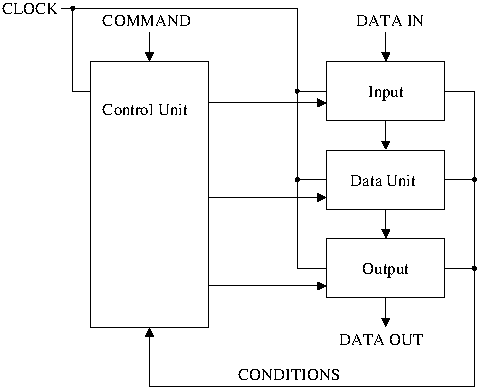
\includegraphics{SynchronousSystemStructure}
  \end{center}
\end{frame}

\section{Synchronous Design Problems}

\subsection{Clock Skew}

\begin{frame}{Just when you thought it was safe...}
  Although synchronous design can eliminate the need to deal with transient signals in components, it does not isolate us completely from analog problems.
  \begin{block}{Light is too slow!}
    The speed of light is finite and unchanging, so it does not reach each component in a circuit at the same time.
  \end{block}
  A complex circuit may have long paths, so the clock may be delayed in some parts of the circuit.
\end{frame}

\begin{itemize}
  \item Using an automatically generated PCB can make this problem worse, as the designer may not know the trace lengths.
  \item Aligning the components in a tree structure can help.
\end{itemize}

\subsection{Asynchronous Inputs}

\begin{frame}{You do not operate on a clock}
  Most inputs to a system are not synchronized to the clock.
  \begin{itemize}
    \item Keyboard, mouse input
    \item Data from an external device (e.g. a GPS signal)
  \end{itemize}
  How can we synchronize these asynchronous inputs?
\end{frame}

\begin{frame}{Synchronizer}
  \begin{center}
    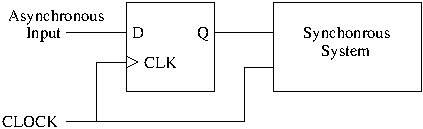
\includegraphics{Synchronizer}
  \end{center}
\end{frame}

\end{document}
